\documentclass[10pt,a4paper]{article}

\usepackage[utf8]{inputenc}
\usepackage[T1]{fontenc}

%%%%%%%%%%% Own packages
\usepackage[a4paper, margin=1in]{geometry}
\usepackage{multicol}
\usepackage{lipsum}
\usepackage{natbib}

% Header/footer
\usepackage{fancyhdr}
\pagestyle{fancy}
\renewcommand{\headrulewidth}{0pt}

% Footnotes at bottom of page
\usepackage[bottom]{footmisc}


% Maths
\usepackage{physics}
\usepackage{esdiff}
\usepackage{cancel}
\usepackage{amstext,amsbsy,amssymb,mathtools}
\usepackage{times} 
\usepackage{siunitx}
\usepackage{tensor}

%% Graphics
\usepackage{caption}
\captionsetup{margin=20pt,font=small,labelfont=bf}
%\renewcommand{\thesubfigure}{(\alph{subfigure})} % Style: 1(a), 1(b)
%\pagestyle{empty}
\usepackage{graphicx} % Include figure files

% Listsings and items
\usepackage[page]{appendix}
\usepackage[shortlabels]{enumitem}
\setenumerate{wide,labelwidth=!, labelindent=0pt}
\usepackage{varioref}
\usepackage{hyperref}
\usepackage{cleveref}

% Paragraph indent and skip
\setlength{\parindent}{2em}
\setlength{\parskip}{1em}
\setlength\extrarowheight{5pt}

%% User units
\DeclareSIUnit \parsec {pc}

%% User commands
\providecommand{\qwhere}
{
    \ensuremath{
    ,\quad \text{where} \quad 
    }
}

\title{AST5220 Cosmology \rm{II}\\ 
\vspace{5mm}Milestone 2 - The Recombination History}
\author{Jakob Borg}
%%%%%%%
\begin{document}
%%%%%%%
\maketitle
\lhead{Milestone 2 AST5220}
\rhead{Jakobbor}
%%%%%%%%
 
\section{Brief Introduction}
The goal of this second milestone\footnote{Second of four milestones.} is to compute what happens during and after the short period of the early universe called recombination. In this period the primordial plasma of free electrons and protons combined into neutral hydrogen. We also want to compute how rapidly this transition happened. To achieve this we will solve the Boltzmann equation for the number density of electrons, using the Saha approximation and Peebles equation.

The main results from these calculations are the optical depth and its first and second derivatives, as well as the visibility function and its derivatives, as functions of the logarithmic scale factor $x$. Using these expressions we will be able to find the time when the cosmic microwave background (CMB) was released from the opaque primordial plasma, defining the so called surface of last scattering where the Universe became transparent.

%The final Because we want to study the CMB.

\subsection{Note on previous milestones}
As mentioned this is part two of four in this overarching project. We will therefore build upon the theory and results from milestone 1\citep{milestone1}, describing the background evolution of the Universe, without further elaboration. One point we would like to mention that is adjusted in the code used from milestone 1 is the initial condition for the conformal time. We now use the more accurate approach
\begin{equation*}
    \eta(x_{start}) = \frac{c}{\mathcal{H}(x_{start})}.
\end{equation*}

%%%%%%%%%%
% Theory
%%%%%%%%%%
\section{Theoretical Background}
\label{sec:Theory}

%%%%%%%%%
\subsection{The Model In Use}
\label{subsec:Theory/Model}
As mentioned, the main results we are interested in are the optical depth and the visibility function (...). In our cosmological model the main source absorbing and disrupting photons are Thompson scattering with free electrons. We will model the optical depth simply according to this kind of scattering alone. Therefore, to calculate these quantities, we need the electron number density.

We are modeling the early Universe as a hot, relativistic primordial plasma with photons, and free electrons and free protons as its only ordinary matter components. That is we exclude helium and any other heavier elements, as well as neutrinos\footnote{To be clear, neutrinos are not  considered a matter component, but is also excluded from our model.}.
After the recombination process we assume we are left in a cool Universe with only hydrogen and photons, and a tiny amount of free electrons left. The interactions between particle species governing this transition, and hence their distributions, are described with the Boltzmann equation, which will be discussed next in \cref{subsec:Theory/Boltzmann eq}.

To clarify, the model still includes the dark matter and dark energy components, which is important for the background evolution computed in milestone 1, but is not important for the interactions modeled during recombination. The dark energy component, modeled as the cosmological constant, is only affecting the expansion of the Universe and is therefore not directly included in the interactions between particle species. The dark matter component could theoretically be included in some type of interaction with it self or other particles, but is not modeled that way here and the component is left unchanged.

%%%%%%%%%%
\subsection{The Boltzmann Equation}
\label{subsec:Theory/Boltzmann eq}
The Boltzmann equation can be written on the following form taken from \cite[p. 61]{Dodelson} describing the number density of particle species $1$, in a process going both ways where species $1$ and $2$ interact and produce species $3$ and $4$
\begin{gather}
    1+2  \rightleftharpoons 3+ 4 \notag
    \\
    \frac{1}{a^3}\diff{a^3n_1}{t} = - \langle \sigma v \rangle \left[n_1n_2 - \left(\frac{n_1n_2}{n_3n_4}\right)_{\rm{EQ}}n_3n_4\right].
    \label{eq:Boltzmann species}
\end{gather}
Here $n_i$ and $\left(n_i\right)_{\rm{EQ}}$ are the mentioned number densities and the known\footnote{Also found in \cite[p. 61]{Dodelson}.} equilibrium (EQ) solutions of the different number densities respectively. While $\langle \sigma v \rangle$ is the thermally averaged cross sections of the interactions, taken from quantum field theory. This equation is permutable in the indices so that it can be written for species $2$, $3$ and $4$ as well. We will apply this equation to our model 
\begin{equation}
    \quad e^{-} + p^{+} \rightleftharpoons H + \gamma,
    \label{eq:process}
\end{equation}
where the processes taking place are as follows. On the left side we have free electrons and protons combining into neutral hydrogen and a photon. On the right side a high energy photon interacts through Compton scattering with a bound electron in a hydrogen atom, ionizing the atom and producing a free electron and proton.

%Under a set of assumptions, described in the following, 
The Boltzmann equation can be rewritten, again following \cite{Dodelson}, into the Saha equation and Peebles equation described in the following (...), which we will use to compute how the number density of free electrons evolve. First we set up some of the more straight forward assumptions. The photons of course stay relativistic always, and so we can approximate their number density by the equilibrium solution $n_\gamma \approx n_\gamma^{\rm{EQ}}$. We also assume that the Universe is neutral, so that $n_e = n_p$. 

\subsubsection{Natural Units}
\label{subsubsec:Theory/natural units}
We have to mention that all the equations listed in \cite{Dodelson} are given in so called natural units, where the familiar constants $\hbar = c = k_b \equiv 1$. These constants are therefore neglected in the equations in the book. In all our calculations we use SI-units, and we must therefore rewrite the equations into proper form with the constants included. This is done through dimensional analyses. This is straight forward, but a bit tedious, and we therefore does not included all the analysis for all the equations to follow. Instead we present one example of how this is done in \cref{asec:Dimensional analysis}.

%Approaching recombination the temperature drops below the non relativistic limit, $m_i >> T$, so we can use the non relativistic solutions for the equilibrium number densities \citep{Dodelson}


\subsection{The Saha Approximation and Equation}
\label{subsubsec:THeory/Saha approximation and equation}
In the early radiation dominated Universe, the plasma was dense and hot with high interaction rates so all the species $i$ are considered to be in EQ
\begin{equation*}
    \diff{a^3n_i}{t} = 0 \quad \Rightarrow \quad \frac{n_e n_p}{n_H n_\gamma} = \left(\frac{n_e n_p}{n_H n_\gamma}\right)_{\rm{EQ}}.
\end{equation*}
As the Universe expands and the temperature and interaction rates drops, the species will gradually fall out of EQ. Thus the number densities for the different species will start to evolve differently. Initially this can be modeled with the Saha approximation
\begin{equation}
    \frac{n_e n_p}{n_H n_\gamma} \approx \left(\frac{n_e n_p}{n_H n_\gamma}\right)_{\rm{EQ}}
    \label{eq:Saha approximation}
\end{equation}
when the species are very close to following their equilibrium distributions. Defining the free electron fraction, $X_e$, as the electron number density over the baryon number density, we can define the Saha equation
\begin{align}
    \frac{X_e^2}{1-X_e} &= \frac{1}{n_b}\left(\frac{m_e k_b T_b}{2\pi \hbar^2}\right)^{3/2} \exp(-\frac{\epsilon_0}{k_b T_b}) \label{eq:Saha equation}
    \\
    \text{where} \quad X_e &= \frac{n_e}{n_b} = \frac{n_e}{n_p+n_H}, \quad X_e \in \left[0,\, 1\right], \label{eq:Free electron fraction}
    \\
    n_b &= \frac{\Omega_{B,0} \rho_{c,0}}{m_H}\exp(-3x) \quad \text{is the baryon number density\footnotemark,} \label{eq:baryon number density}
    \\
    \text{and} \quad \epsilon_0 &= \left(m_e + m_p - m_h\right)c^2 = \SI{13.6}{eV} \quad \text{is the binding energy of hydrogen.} \notag
\end{align}
\footnotetext{known from milestone 1.}%
\Cref{eq:Saha equation} is valid for as long as the Saha approximation holds, quantitatively for as long as $X_e \approx 1$\footnote{Note that the free electron fraction of course starts at $X_e=1$ in the primordial plasma.}. The temperature involved is specifically the temperature of the baryons. Here we employ another approximation, which is reasonable to a large degree considering all our other approximations, that the baryon temperature follow the radiation temperature
\begin{equation}
    T_b(x) = T_r(x) = T_{\rm{CMB}}(x=0)\exp(-x)
\end{equation}
where the temperature of the CMB today is $T_{\rm{CMB}}(x=0) = \SI{2.725}{K}$. We will therefore just note the temperature as $T$ from now on, referring to the baryon and radiation temperature as a function of the logarithmic scale factor.

\subsection{The Peebles Equation}
\label{subsec:Theory/Peebles equation}
Going beyond the equilibrium solutions we can no longer assume the species to follow the Saha approximation, \cref{eq:Saha approximation}. The Saha equation, \cref{eq:Saha equation}, predicts the outset of recombination pretty accurately, but fails miserably for the evolution of the electron density as the system goes out of equilibrium. We will here employ the Peebles equation, describing the free electron fraction according to the Boltzmann equation with the relevant interactions included in our model. These are combinations of free electrons and protons into hydrogen in its first or higher order excited states. Recombinations into the ground state is not included as this will also produce a photon with high enough energy to ionize another hydrogen atom in its ground state, resulting in a zero net change in the number densities. The Peebles equation goes as follows 


\begin{equation}
\diff{X_e}{x} = \frac{C_r(T)}{H(x)} \left[\beta(T)(1-X_e) - n_H
\alpha^{(2)}(T)X_e^2\right],
\label{eq:Peebles equation}
\end{equation}
where
\begingroup
\allowdisplaybreaks
\begin{align}
C_r(T) &= \frac{\Lambda_{2s\rightarrow1s} +
\Lambda_{\alpha}}{\Lambda_{2s\rightarrow1s} + \Lambda_{\alpha} +
\beta^{(2)}(T)},
\\
\Lambda_{2s\rightarrow1s} &= 8.227 \textrm{s}^{-1},
\\
\Lambda_{\alpha} &= \frac{H(x)}{(8\pi)^2 n_{1s}} \left(\frac{3\epsilon_0}{\hbar c}\right)^3,
\\
n_{1s} &= (1-X_e)n_H,
\\
\beta^{(2)}(T) &= \beta(T) \exp(\frac{3\epsilon_0}{4k_b T}), \label{eq:beta 2}
\\
\beta(T) &= \alpha^{(2)}(T) \left(\frac{m_e k_b T}{2\pi\hbar^2}\right)^{3/2} \exp(-\frac{\epsilon_0}{k_b T}), \label{eq:beta}
\\
\alpha^{(2)}(T) &= \frac{64\pi}{\sqrt{27\pi}} \sigma_T c \sqrt{\frac{\epsilon_0}{k_b T}}\phi_2(T),
\\
\sigma_T &= \frac{8\pi}{3}\frac{\alpha^2\hbar^2}{m_e^2c^2}, \label{eq:sigma T}
\\
\phi_2(T) &= 0.448\ln(\frac{\epsilon_0}{k_b T}). \label{eq:phi Peebles}
\end{align}
\endgroup
and $H(x)$ is the Hubble parameter, discussed in detail in \cite{milestone1}.
%\hfill

\subsection{The Optical Depth and Visibility Function}
\label{subsec:Theory/tau and g}
The optical depth describes how much the intensity of incident light that moves a distance $x$ through a medium will be reduced by absorption, quantitatively as $I(x) = I_0 \exp(-\tau)$ where $I_0$ is the intensity emitted at the source. As mentioned, in our model we look at absorption through Thompson scattering alone. The optical depth is then defined as
\begin{equation}
    \tau(x) = \int_x^{x_{\rm{Today}=0}} \frac{\sigma_T n_e c}{H(x)}\dd{x}
    \label{eq:tau integration}
\end{equation}
where $\sigma_T$ is the Thompson cross section defined in \cref{eq:sigma T}. The electron number density can be obtained using the free electron fraction from the Saha and Peebles equations multiplied by the baryon number density. There are two interesting regimes governed by the optical depth. If $\tau \gg 1$ we say the medium is optically thick, and thus the intensity $I(x)$ will be approximately zero. The other way around, if $\tau \ll 1$ the medium is optically thin, and $I(x) \approx I_0$. When $\tau  = 1$ is usually used to define the transition between these two regimes, and can be thought of as when the medium goes from opaque to transparent.

With the optical depth we can also define the visibility function
\begin{equation}
    \tilde{g}(x) = - \diff{\tau}{x}\exp(-\tau) = -\tau^\prime \exp(-\tau)
    \label{eq:visibility function}
\end{equation}
where we have used the $\tau^\prime$ notation for the derivative with respect to the logarithmic scale factor. We will continue to use this through the report where it is convenient. \Cref{eq:visibility function} is a probability distribution, in the sense that $\int_{-\infty}^0 \tilde{g}\dd x = 1$. We interpret this function as the probability that a photon last scattered at time $x$, going backwards in time from today.

%%%%%%%%
% Method
%%%%%%%%
\section{Method}
\label{sec:Method}
As mentioned, this milestone builds upon the work done in milestone 1\citep{milestone1}, calculating everything we need for the background cosmology. These calculations are performed by the class \textit{BackgroundCosmology}. The work in this milestone is carried out by the class \textit{RecombinationHistory}, which takes as input an instance of the mentioned \textit{BackgroundCosmology} class with all the required calculations already done\footnote{The class also takes as input the helium fraction, but this is set to zero and does not contribute anything.}.

With the equations we need defined in \cref{sec:Theory} we can now describe our approach step for step to solve for the optical depth and the visibility functions and their derivatives.

\subsection{Solving the Saha and Peebles equations}
\label{subsec:Method/Solving Xe}
First we implemented a method to get the baryon number density at time $x$, using \cref{eq:baryon number density}. This is used in both \cref{eq:Saha equation,eq:Peebles equation}, as well as solving for the electron number density once we have the free electron fraction.

Next we solve for the free electron fraction using \cref{eq:Saha equation,eq:Peebles equation} in an x-interval from $-12$ to $2$ with $\num{1e5}$ points. Here we have to consider multiple numerical stability issues. First we must define a transition between the two regimes for when the Saha equation is no longer valid, due to the Saha approximation being validated, and define this as when $X_e < 0.99$. Looking at \cref{eq:Saha equation}, this is a simple quadratic equation in $X_e$, which we solve as follows
\begin{align*}
    \text{let} \quad  F &\equiv \frac{1}{n_b}\left(\frac{m_e k_b T_b}{2\pi \hbar^2}\right)^{3/2} \exp(-\frac{\epsilon_0}{k_b T_b})
    \\
    \text{then} \quad X_e &= \frac{-F \pm \sqrt{F^2 + 4F}}{2} = \frac{-F + F\sqrt{1+\frac{4}{F}}}{2}
\end{align*}
where we have used the positive solution as $X_e$ can not be negative. In the early universe the temperature was extremely high and thus $F$ is a huge number. This is a numerical issue, essentially we subtract a huge number from a huge number, which is unstable. We solve this by Taylor expanding the square root to the first order so the solution is well defined
\begin{align*}
    \sqrt{1+\frac{4}{F}} &\approx 1+ \frac{2}{F}
    \\
    \Rightarrow \quad \frac{-F + F\sqrt{1+\frac{4}{F}}}{2} &\approx \frac{-F + F +2}{2} = 1.
\end{align*}
We also want to compare the solution from using the more accurate approximation with the Peebles equation with the solution obtained through the Saha equation alone. Thus we have a problem later on, when the temperature drops and $F$ goes to zero so $4/F$ diverges. This is all solved in the code by implementing it as follows
\begin{align*}
    X_e = \begin{cases}
        \num{1} &\qif F > \num{1e9}
        \\
        \num{1e-20} &\qif F < \num{1e-20}
        \\
        \frac{-F + F\sqrt{1+\frac{4}{F}}}{2}  &\quad \text{else}
    \end{cases}
\end{align*}
where the exact thresholds for each regime is found through experimentation. Note that we don't set the solution to zero, but a very small number, when $F$ is small. This is because we want to create splines of the logarithmic results in the end, as the logarithmic $X_e$ varies smoother in $x$.

We solve the Saha equation in the full time interval, to have this solution to compare our more accurate solution with later, but we keep track of the exact index $x_i$ of our time array where our $X_e< 0.99$ condition is met, and what value we have for $X_e$ at this point, $X_{e,i}$. This is used in the following for solving the Peebles equation, \cref{eq:Peebles equation}, which is an ordinary differential equation (ODE).

To solve the Peebles equation, we use the class \textit{ODESolver} wrapping the GSL library providing multiple ODE algorithms. We chose specifically the well known explicit embedded Runge-Kutta-Fehlberg (4, 5) method\citep{gsl-doc}. To solve the system we use the mentioned recorded $X_{e,i}$ as initial condition, and create a new time array spanning from the time corresponding to the index $x_i$, $x_{\rm{Peebles}} \in \left[x(x_i),\, 2\right]$. When implementing the \crefrange{eq:Peebles equation}{eq:phi Peebles} we have to take care of the exponential in \cref{eq:beta 2}. When the temperature drops to a low value this will diverge out of control. Therefore we implement \cref{eq:beta 2} writing out the full expression for \cref{eq:beta} so we can combine the two exponential terms
\begin{equation*}
    \beta^{(2)} = \alpha^{(2)}(T) \left(\frac{m_e k_b T}{2\pi\hbar^2}\right)^{3/2} \exp(-\frac{\epsilon_0}{4k_b T}).
\end{equation*}

As briefly mentioned, the logarithmic results from both the combined Peebles and Saha solution and the Saha solution alone are splined, as well as the logarithmic electron number density using \cref{eq:Free electron fraction}. These splines are used in the following when we need the electron number density, and so we implement a get method to easily convert back and fourth from the logarithmic and normal value.

\subsection{Solving for the Optical Depth and Visibility Function}
\label{subsec:method/tau and g}
We solve for the optical depth and visibility function in the same time interval as in \cref{subsec:Method/Solving Xe} with the same number of points. Here we prepare to solve for both quantities, and their first derivatives. First we rewrite \cref{eq:tau integration} into an ODE
\begin{equation}
    \diff{\tau }{x} = -\frac{\sigma_t n_e c}{H(x)}
    \label{eq: tau ODE}
\end{equation}
and solve it with the same algorithm as we did for the Peebles equation. We don't know the initial condition for this equation, but we do know the numerical value of it today\footnote{Or in other words at our location, distance $x=0$ away.} at $x=0$. We therefore chose one arbitrary and large initial value, $\tau_{\rm{init}} = \num{1e3}$, and then normalized the result in the end by subtracting the computed value of $\tau(x=0)$ from every grid point. To do this we find the index where $x=0$ dynamically, call it $x_{\rm{zero}}$.

The first derivative of $\tau$ is obtained directly through the ODESolver, and before we normalize the optical depth we create the spline for this derivative. Using this spline we can fetch the second derivative too. This way we can use the spline to compute the first derivative of the visibility function, all in the same loop as we are normalizing the optical depth and computing the visibility function it self. To do this we use the chain rule on \cref{eq:visibility function} to express it analytically, and compute the quantities according to this scheme
\begin{align*}
    \text{for } i \in &[0,n-1]:
    \\
    \bar{\tau}_i &= \tau_i - \tau_{x_{\rm{zero}}}
    \\
    \tilde{g}_i &= - \diff*{\tau}{x}{i}\exp(-\bar{\tau}_i)
    \\
    \tilde{g}_i^\prime &= \left[\left(\diff*{\tau}{x}{i}\right)^2-\diff*[2]{\tau}{x}{i}\right]\exp(-\bar{\tau}_i)
\end{align*}
where $\tilde{g}_i^\prime$ is the first derivative of the visibility function with respect to $x$, subscripts indicate the grid point the quantities are evaluated at, and $n$ is the number of points. $\diff[2]{\tau}{x}$ is obtained through the spline of $\diff{\tau}{x}$ which we prepared before the loop.

In the end, we create splines of $\tau$, $\tilde{g}$ and $\tilde{g}^\prime$. As mentioned, the second derivative of $\tau$ is obtained through the spline of $\tau^\prime$. Likewise for the second derivative of the visibility function, it is obtained through the spline of $\tilde{g}^\prime$. All the splines are then implemented into convenient get methods in the class.

The last thing we want to compute is the specific times where we 

%%%%%%%%
%Results
%%%%%%%%
\section{Results}
\label{sec:Results}


\begin{figure}[ht]
    \centering
    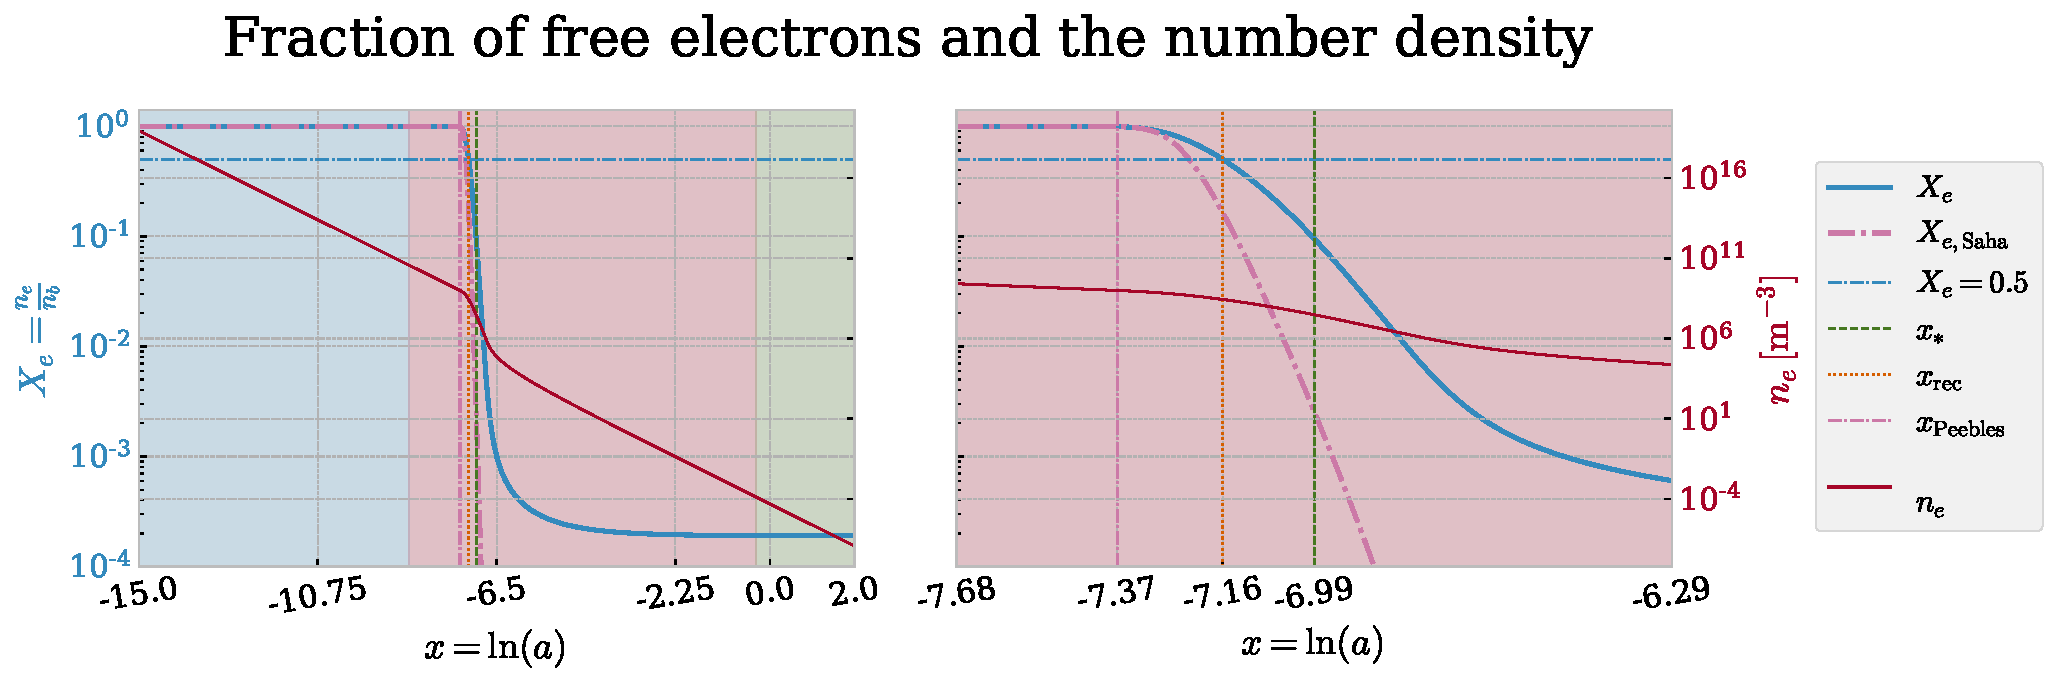
\includegraphics[scale=0.5]{../figs/free_electrons.pdf}
    \caption{Plot showing the free electron fraction $X_e$, left y-axis, and electron number density $n_e$, right y-axis. The solution obtained using only Saha equation is included in the pink dash-dotted line, $X_{e,\rm{Saha}}$, which drops off exponentially to zero once the solution deviates from equilibrium. The horizontal blue dashed line at $X_e=0.5$ indicate where recombination is half-way done, at $x\approx-7.16\equiv x_{\rm{rec}}$. The surface of last scattering is indicated at $x\approx-6.99\equiv x_{\rm{\star}}$. The left panel zoom in centered on $x_{\star}$, showing a $\SI{10}{\%}$ buffer in $x$ on both sides.}
    \label{fig:Xe and ne}
\end{figure}

\begin{figure}[ht]
    \centering
    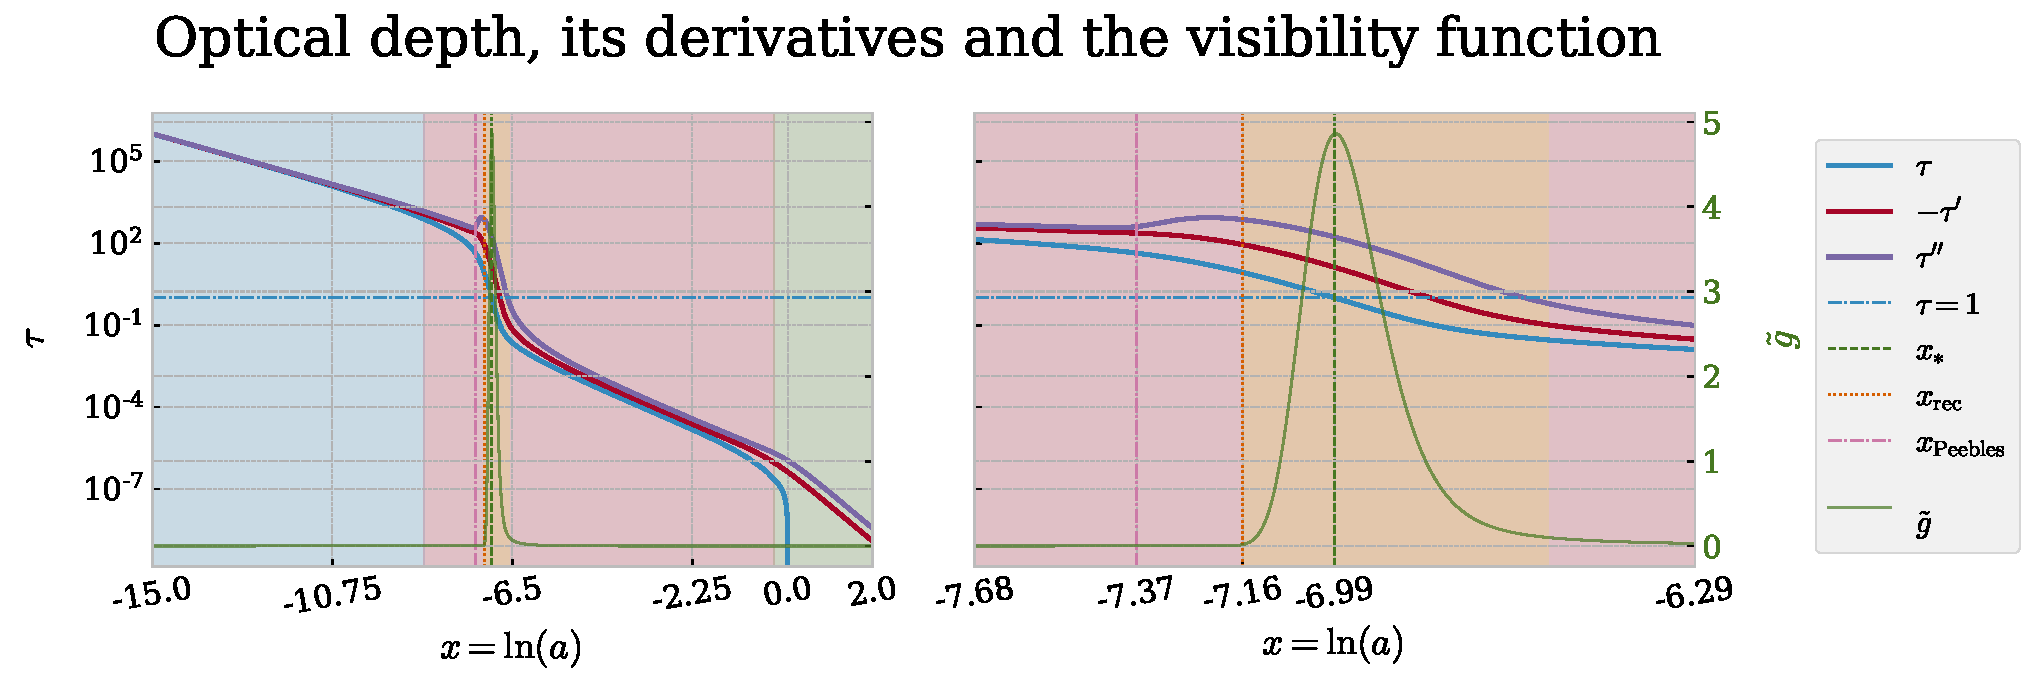
\includegraphics[scale=0.5]{../figs/optical_depth.pdf}
    \caption{Plot showing the optical depth and its two first derivatives, left y-axis, and the visibility function, right y-axis. $x\approx-7.16\equiv x_{\rm{rec}}$ indicate where recombination is half-way done. The surface of last scattering is indicated at $x\approx-6.99\equiv x_{\rm{\star}}$, located at the peak in $\tilde{g}$ and where $\tau=1$. The left panel zoom in centered on $x_{\star}$, showing a $\SI{10}{\%}$ buffer in $x$ on both sides.}
    \label{fig:tau}
\end{figure}

\begin{figure}[ht]
    \centering
    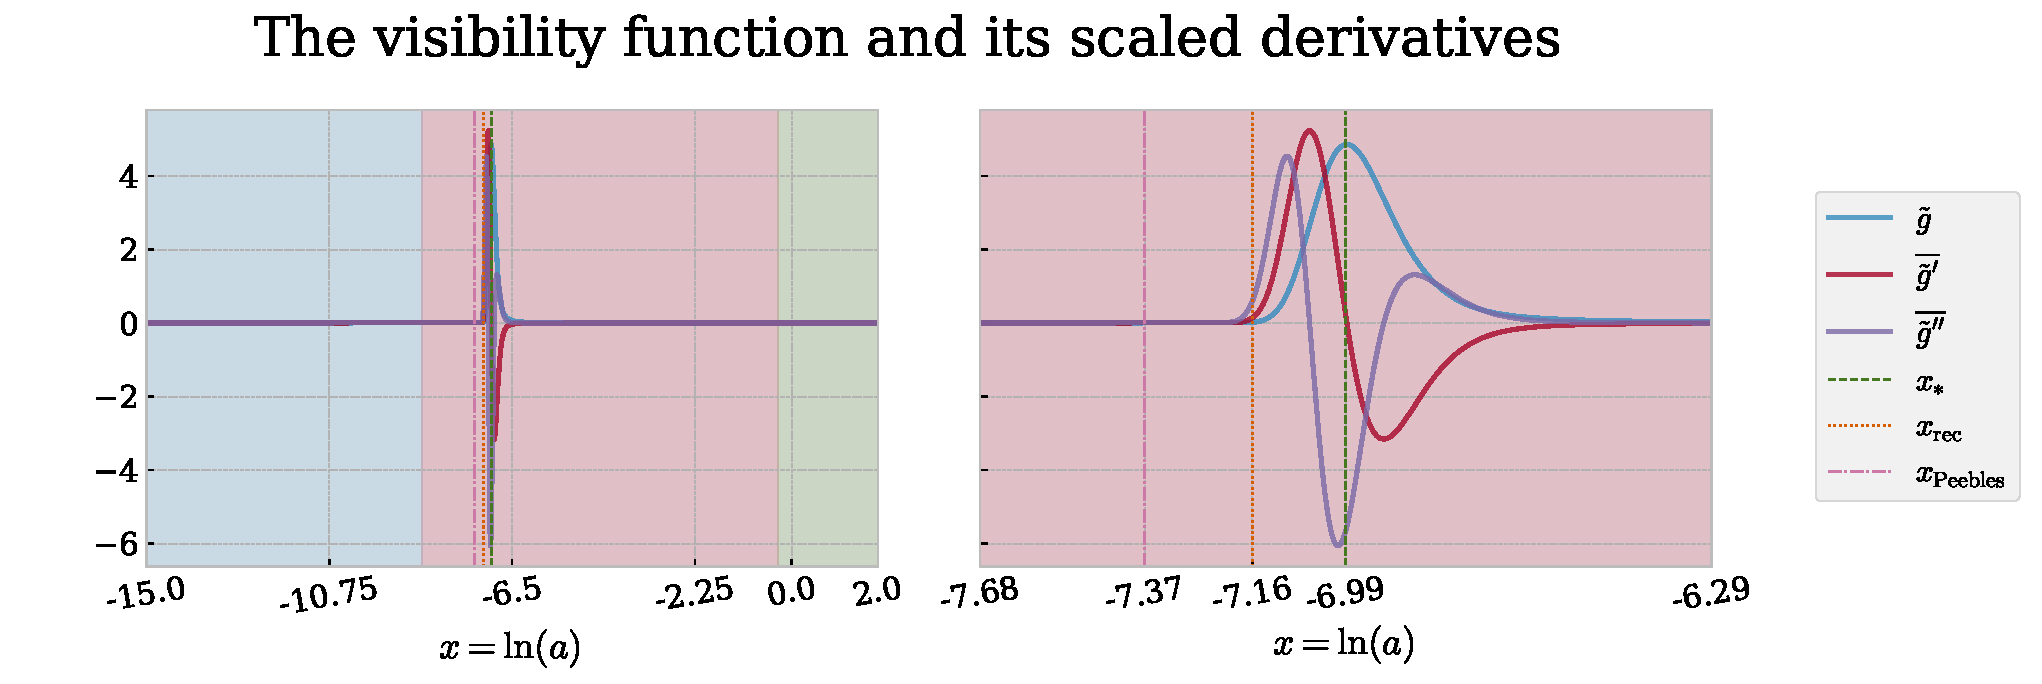
\includegraphics[scale=0.5]{../figs/visibility_functions.pdf}
    \caption{Plot showing the visibility function and its two first derivatives, all scaled}
    \label{fig:g}
\end{figure}

% \section{Notes}
% Derivative of tau corresponds to interaction rate relative to the expansion rate.
\pagebreak
\bibliographystyle{plainnat}
\bibliography{ref_milestone2}

\clearpage
\begin{appendices}
    \appendix

    \section{Dimensional Analysis of the Saha Equation}
    \label{asec:Dimensional analysis}
    Here follows an example of how to perform the dimensional analysis to rewrite the Saha equation as listed in \cite[p. 70]{Dodelson} in natural units into the form of \cref{eq:Saha equation}. First we do one simplifying step. As we neglect the helium atoms and assume a neutral universe we can write the sum of electron and hydrogen number densities as the baryon density, $n_e + n_H = n_p + n_H = n_b$.
    \begin{equation*}
        \text{Original form} \quad 
        \underbrace{\frac{X_e^2}{1-X_e}}_{\rm{[Unitless]}} = \underbrace{\frac{1}{n_b}}_{[\si{m^3}]}\underbrace{\left(\frac{m_e T_b}{2\pi}\right)^{3/2}}_{[\si{kg^{3/2}.K^{3/2}}]} \underbrace{\exp(-\frac{m_e+m_p-m_H}{T_b})}_{\exp([\si{kg.K^{-1}}])}
    \end{equation*}
    We must now balance the equation to get the right units on the left hand side of the equation. That is we must make the equation unitless. First, we have to remove the units inside the exponential function. Here we recognize the nominator as the binding energy of hydrogen, if we multiply with a factor $c^2$, thus the nominator is in units joule. To make the denominator have the same units we multiply with the Boltzmann constant.
    \begin{equation*}
        \frac{\left(m_e+m_p-m_H\right)c^2}{k_b T_b} = \frac{\epsilon_0}{k_b T_b} \quad \Rightarrow \quad \frac{[\si{J}]}{[\si{J.K^{-1}.K}]} = [\rm{Unitless}]
    \end{equation*}
    Next we have to make the product in front of the exponential unitless as well. The simplest way to do this is to pull the baryon number density inside the parenthesis, and then avoid the exponent $3/2$ all together.
    \begin{equation*}
        \frac{1}{n_b}\left(\frac{m_eT_b}{2\pi}\right)^{3/2} \quad \Rightarrow \quad \underbrace{\left(\frac{m_e T_b}{n_b^{2/3}}\right)}_{[\si{kg.K.m^2}]}
    \end{equation*}
    To get rid of the temperature we need the Boltzmann constant, but we then introduce units of energy. To remove the unit of energy and the left unit of mass we need the square of the Planck constant.
    \begin{equation*}
        \left(\frac{m_e k_b T_b}{n_b^{2/3}\hbar^2}\right) \quad \Rightarrow \quad \frac{[\si{kg.K.m^2.J}]}{[\si{K.J^2.s^2}]} = \frac{[\si{kg.m^2}]}{[\si{s^2}]}\frac{1}{[\si{J}]} = [\rm{Unitless}]
    \end{equation*}
    Now we have the equation on its proper SI-unit form, as in \cref{eq:Saha equation}
    \begin{equation*}
        \frac{X_e^2}{1-X_e} = \frac{1}{n_b}\left(\frac{m_e k_b T_b}{2\pi \hbar^2}\right)^{3/2} \exp(-\frac{\epsilon_0}{k_b T_b}).
    \end{equation*}

\end{appendices}

\end{document}